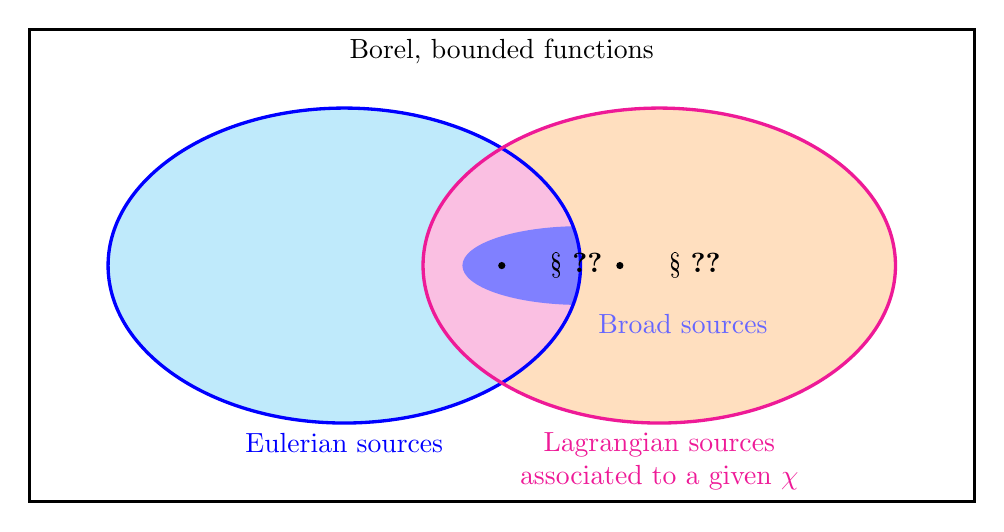
\begin{tikzpicture}[x=1cm,y=1cm]
  % frame and title
  \draw[line width=1.2pt] (0,0) rectangle (12,6);
  \node at (6,6) [below] {Borel, bounded functions};

  % base fills
  \fill[cyan!25]   (4,3) ellipse (3 and 2); % Eulerian
  \fill[orange!25] (8,3) ellipse (3 and 2); % Lagrangian for given chi

  % intersection tint
  \begin{scope}
    \clip (4,3) ellipse (3 and 2);
    \fill[magenta!25] (8,3) ellipse (3 and 2);
  \end{scope}

  % broad sources: only inside the intersection
  \begin{scope}
    \clip (4,3) ellipse (3 and 2);
    \clip (8,3) ellipse (3 and 2);
    \fill[blue!50] (7,3) ellipse (1.5 and 0.5);
  \end{scope}
  \node[text=blue!60] at (8.3,2.5) [below, align=left] {Broad sources};

  % outlines on top
  \draw[blue, line width=1.2pt]        (4,3) ellipse (3 and 2);
  \draw[magenta!90, line width=1.2pt]  (8,3) ellipse (3 and 2);

  % labels
  \node[text=blue] at (4,1) [below] {Eulerian sources};
  \node[text=magenta!90, align=center] at (8,1) [below]
    {Lagrangian sources\\ associated to a given $\chi$};

  % reference markers
  \fill (6,3) circle (1.3pt);
  \node[anchor=west] at (6.5,3) {\S~\ref{S:compatibilitysources}};
  \fill (7.5,3) circle (1.3pt);
  \node[anchor=west] at (8,3) {\S~\ref{S:Cantoparam}};
\end{tikzpicture}